\documentclass[9pt]{beamer}
\usetheme{boxes}
\usetheme{Boadilla}
\usecolortheme{beaver}
%\usecolortheme{sidebartab}
% \usefonttheme{structurebold}
\usefonttheme{serif}

%gets rid of bottom navigation bars
\setbeamertemplate{footline}[page number]{}

%gets rid of navigation symbols
\setbeamertemplate{navigation symbols}{}


% \usepackage{helvet}
\usepackage{amsmath, amssymb}
\usepackage{color}
%\usepackage{asymptote}
\usepackage{mathrsfs}
\usepackage{dsfont}
\usepackage{url}
\usepackage{cancel}
\usepackage{tikz}
\usetikzlibrary{fit,positioning}
\usetikzlibrary{shapes,matrix,decorations.markings,arrows}
\usetikzlibrary{graphs}
\usepackage{bbm}
\def\ind{\mathbbm{1}} %Indicator function


%
\definecolor{darkblue}{rgb}{0.0, 0.0, 0.55}
\setbeamercolor{title}{fg=darkblue}
\setbeamercolor{frametitle}{fg=darkblue}
\newcommand{\myitem}{\item[$\bullet$]}
\definecolor{darkgreen}{rgb}{0, 0.55, 0}


\newcommand{\LABEQ}[1]{\label{eq:#1}}%\mathtt{[eq:#1]}\qquad
\newcommand{\LABALG}[1]{\label{alg:#1}}%\mathtt{[lab:#1]}\qquad
\newcommand{\LABTAB}[1]{\label{tab:#1}}%{\tt [tab:$\text{$#1$}$]}}
\newcommand{\LABFIG}[1]{\label{fig:#1}}%{\tt [fig:$\text{$#1$}$]}}
\newcommand{\LABTHM}[1]{\label{thm:#1}}%{\tt [thm:#1]}}
\newcommand{\LABPRP}[1]{\label{prp:#1}}%{\tt [prp:#1]}}
\newcommand{\LABLEM}[1]{\label{lem:#1}}%{\tt [lem:#1]}}
\newcommand{\LABCOR}[1]{\label{cor:#1}}%{\tt [cor:#1]}}
\newcommand{\LABDFN}[1]{\label{dfn:#1}}%{\tt [dfn:#1]}}
\newcommand{\LABFNT}[1]{\label{fnt:#1}}%{\tt [fnt:#1]}}
\newcommand{\EQ}[1]{\eqref{eq:#1}}%$^{\text{\tt [#1]}}$} %used to be  %{(\ref{eq:#1})}
\newcommand{\ALG}[1]{~\ref{alg:#1}}
\newcommand{\TAB}[1]{~\ref{tab:#1}}%$^{\text{\tt [#1]}}$}
\newcommand{\FIG}[1]{\ref{fig:#1}} %$^{\text{\tt [#1]}}$}
\newcommand{\THM}[1]{~\ref{thm:#1}}%$^{\text{\tt [#1]}}$}
\newcommand{\COR}[1]{~\ref{cor:#1}}%$^{\text{\tt [#1]}}$}
\newcommand{\PRP}[1]{~\ref{prp:#1}}%$^{\text{\tt [#1]}}$}
\newcommand{\LEM}[1]{~\ref{lem:#1}}%$^{\text{\tt [#1]}}$}
\newcommand{\DFN}[1]{~\ref{dfn:#1}}%$^{\text{\tt [#1]}}$}
\newcommand{\FNT}[1]{~\ref{fnt:#1}}%$^{\text{\tt [#1]}}$}
\newcommand{\PAGEEQ}[1]{~\pageref{eq:#1}}
\newcommand{\PAGETAB}[1]{~\pageref{tab:#1}}
\newcommand{\PAGEFIG}[1]{~\pageref{fig:#1}}
\newcommand{\LABCHAP}[1]{\label{chap:#1}}%{\tt [chap:#1]}}
\newcommand{\LABSEC}[1]{\label{sec:#1}}%{\tt [sec:#1]}}
\newcommand{\LABSSEC}[1]{\label{ssec:#1}}%{\tt [ssec:#1]}}
\newcommand{\LABSSSEC}[1]{\label{sssec:#1}}%{\tt [sssec:#1]}}
\newcommand{\CHAP}[1]{~\ref{chap:#1}}%$^{\text{\tt [c:#1]}}$}
\newcommand{\SEC}[1]{~\ref{sec:#1}}%$^{\text{\tt [s:#1]}}$}
\newcommand{\SSEC}[1]{~\ref{ssec:#1}}%$^{\text{\tt [ss:#1]}}$}
\newcommand{\SSSEC}[1]{~\ref{sssec:#1}}%$^{\text{\tt [sss:#1]}}$}



\newcommand{\ve}[1]{\boldsymbol{#1}}
\newcommand{\set}[1]{\mathcal{#1}}

\def\a{\mathtt{a}}
\def\X{\ve{X}}
\def\x{\ve{x}}
\def\y{\ve{y}}
\def\Y{\ve{Y}}
\def\S{\ve{S}}
\def\s{\ve{s}}
\def\n{\mathtt{n}}
\def\C{\mathcal{C}}
\def\H{\ve{H}}
\newcommand{\st}[1]{{e}_{#1}}		%state
\newcommand{\str}[2]{{e}_{#2,(#1)}}	
\newcommand{\St}[1]{{E}_{#1}}		%state
\def\seqst{\ve{\st{}}}
\def\seqSt{\ve{\St{}}}
\def\S{\ve{S}}		%Symbol sequence
\def\AQAM{\mathcal{A}}
\def\Aest{\mathcal{E}}
\def\chl{\mathtt{h}} %Channel length
\def\s{\ve{s}} %transmitted word of symbols
\def\sk{{s}_k} %transmitted word of symbols 
\def\hsk{\hat{\s}_k}
\def\t{\mathtt{s}}   %Word length (symbols)

\newcommand{\p}[1]{p_{_{#1}}} %pdf or pmf
\newcommand{\q}[1]{q_{_{#1}}} %pdf or pmf
\newcommand{\Iset}[1]{\mathtt{#1}} %Index set
\def\d{\text{d}}	%Differential (for integrals)


% Sum Product Algorithm

\newcommand{\mes}[2]{m_{#1\rightarrow#2}}
\newcommand{\logmes}[2]{l_{#1\rightarrow#2}}

\newcommand{\mc}[1]{\mathcal{#1}}
\def\sX{\mc{X}}

\newcommand\Def[1]{{\textbf{Definition:}\\\emph{#1}\\\begin{center} ------------------------ \end{center}}}
\newcommand\Prop[1]{{\textbf{\textcolor{red}{Property:}}\\\emph{#1}\\\begin{center} \textcolor{red}{------------------------} \end{center}}}

\newcommand{\noteB}[1]{\textbf{\textcolor{darkblue}{#1}}}

\newcommand{\noteR}[1]{\textbf{\textcolor{darkred}{#1}}}

\newcommand{\noteG}[1]{\textbf{\textcolor{darkgreen}{#1}}}

\newcommand{\snoteB}[1]{{\textcolor{darkblue}{#1}}}

\newcommand{\snoteR}[1]{{\textcolor{darkred}{#1}}}

\newcommand{\snoteG}[1]{{\textcolor{darkgreen}{#1}}}


\newcommand{\fs}[2]{#2}

\title[]{Inference over discrete FGs with cycles}
\author[\textcolor{white}{Advanced Digital Communications}]{Introduction to Graphical Models and Inference for Communications\\\vspace*{3mm}{\small \textcolor{black}{UC3M}}
}
%\date[08/02/2016]{{08/02/2016}}
\institute{\textcolor{white}{}}

\AtBeginSection[]
{
  \begin{frame}<beamer>{Index}
    \tableofcontents[currentsection,currentsubsection]
  \end{frame}
}

\begin{document}

\frame{
\titlepage
\thispagestyle{empty}
\begin{center}
\includegraphics[scale=0.05]{Figuras/uc3m-logo.pdf}
\end{center}
}

\frame{
\frametitle{Today}

\begin{itemize}
\item We want to perform inference over discrete probability distributions that are represented by  Factor Graphs that are not trees, the graph has cycles!
\end{itemize}
\begin{itemize}
\item \noteR{Exact inference is in general $\mathcal{O}(|\set{X}|^n)$.}
\end{itemize}

\begin{itemize}
\item Approximate Inference using BP!
\begin{itemize}
\item \noteG{Very fast :) ... poor accuracy in general :(}
\item \noteG{In some scenarios the BP accuracy is remarkable!}
\end{itemize}
%\item Almost Exact Inference using MCMC methods (Gibbs sampling/Metropolis Hastings algorithm...)
%\begin{itemize}
%\item \noteG{Slow in very high dimensions :( ... asymptotically exact!  :)}
%\end{itemize}
\end{itemize}

%\begin{block}{Between BP and MCMC methods}
%Deterministic approximate inference methods such as Variational Methods, Expectation Propagation, Generalized BP (Kikuchi approximations) ....
%\end{block}


}

\section{Tools for simple graphs with cycles}
\subsection{Clustering}
\frame{
\frametitle{Clustering}


\begin{align*}
\p{\X}(\x)=\frac{1}{Z} t_1(x_1,x_2) t_2(x_2,x_3,x_4) t_3(x_3,x_5)t_4(x_4)t_5(x_4,x_5), \qquad \x\in\set{X}^5
\end{align*}

\begin{center}
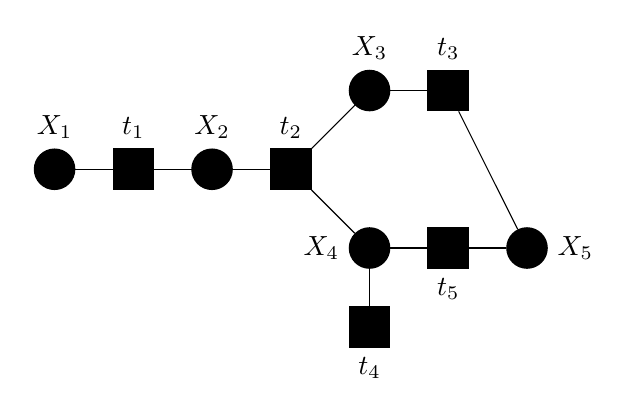
\begin{tikzpicture}[scale=1]
\tikzstyle{factor}=[rectangle,minimum size = 5mm, thick, draw =black,fill=black]
\tikzstyle{var}=[circle,minimum size = 5mm, thick, draw =black,fill=black]
\tikzstyle{second}=[circle, minimum size = 10mm, thick]
\tikzstyle{box}=[rectangle, draw=black!100]
\tikzstyle{connect}=[-latex, thick]
\draw[step=5cm];
	\node[var] (x_1) at (-1,0) [label=above:{$X_1$}]{};
	\node[factor] (t_1) at (0,0) [label=above:{$t_1$}]{};
	\node[var] (x_2) at (1,0) [label=above:{$X_2$}]{};
	\node[factor] (t_2) at (2,0) [label=above:{$t_2$}]{};
	\node[var] (x_3) at (3,1) [label=above:{$X_3$}]{};
	\node[factor] (t_3) at (4,1) [label=above:{$t_3$}]{};
	\node[var] (x_4) at (3,-1) [label=left:{$X_4$}]{};
	\node[factor] (t_4) at (3,-2) [label=below:{$t_4$}]{};
	\node[factor] (t_5) at (4,-1) [label=below:{$t_5$}]{};
	\node[var] (x_5) at (5,-1) [label=right:{$X_5$}]{};
	
	
	\path
		(x_1) edge []  (t_2) 
		(t_2) edge [] (x_3) 
		(x_3) edge [] (t_3)
		(t_2) edge [] (x_4)
		(t_4) edge [] (x_4)
		(x_4) edge [] (x_5)
		(t_3) edge [] (x_5);
		
\end{tikzpicture}
\end{center}



}

\frame{

By defining $\S=[\begin{array}{ccc} X_3 & X_4 & X_5 \end{array}]^T$, the same distribution factorizes as follows 

\begin{align*}
&\p{\X}(\x)=\frac{1}{Z} t_1(x_1,x_2) t_2(x_2,x_3,x_4) \underbrace{t_3(x_3,x_5)t_4(x_4)t_5(x_4,x_5)}_{t_s(\s) }\\\\
&\p{\X}(\x)=\frac{1}{Z} t_1(x_1,x_2) t_2(x_2,\s) t_s(\s)\\\\
&x_3=\left[\begin{array}{ccc}  1 & 0 & 0 \end{array} \right] \s, \qquad 
x_4=\left[\begin{array}{ccc}  0 & 1 & 0 \end{array} \right] \s, \qquad 
x_5=\left[\begin{array}{ccc}  0 & 0 & 1 \end{array} \right] \s,
\end{align*}



}

\frame{

\begin{center}
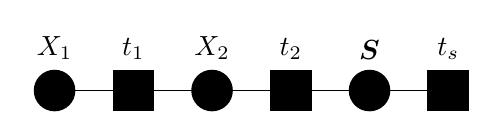
\begin{tikzpicture}[scale=1]
\tikzstyle{factor}=[rectangle,minimum size = 5mm, thick, draw =black,fill=black]
\tikzstyle{var}=[circle,minimum size = 5mm, thick, draw =black,fill=black]
\tikzstyle{second}=[circle, minimum size = 10mm, thick]
\tikzstyle{box}=[rectangle, draw=black!100]
\tikzstyle{connect}=[-latex, thick]
\draw[step=5cm];
	\node[var] (x_1) at (-1,0) [label=above:{$X_1$}]{};
	\node[factor] (t_1) at (0,0) [label=above:{$t_1$}]{};
	\node[var] (x_2) at (1,0) [label=above:{$X_2$}]{};
	\node[factor] (t_2) at (2,0) [label=above:{$t_2$}]{};
	\node[var] (s) at (3,0) [label=above:{$\S$}]{};
	\node[factor] (t_s) at (4,0) [label=above:{$t_s$}]{};
	
	
	\path
		(x_1) edge []  (t_2) 
		(t_2) edge [] (s) 
		 (s) edge [] (t_s);
		
\end{tikzpicture}
\end{center}

\begin{exampleblock}{}
BP is exact!
\end{exampleblock}

\begin{alertblock}{Increased complexity}
Computing the message
\begin{align*}
\displaystyle\mes{t_2}{x_2}(x_2)=\sum_{\s}~ t_j(x_2,\s)t_s(\s)
\end{align*}
requires $\mathcal{O}(|\set{X}|^3)$ operations.
\end{alertblock}


}



\frame{



\begin{center}
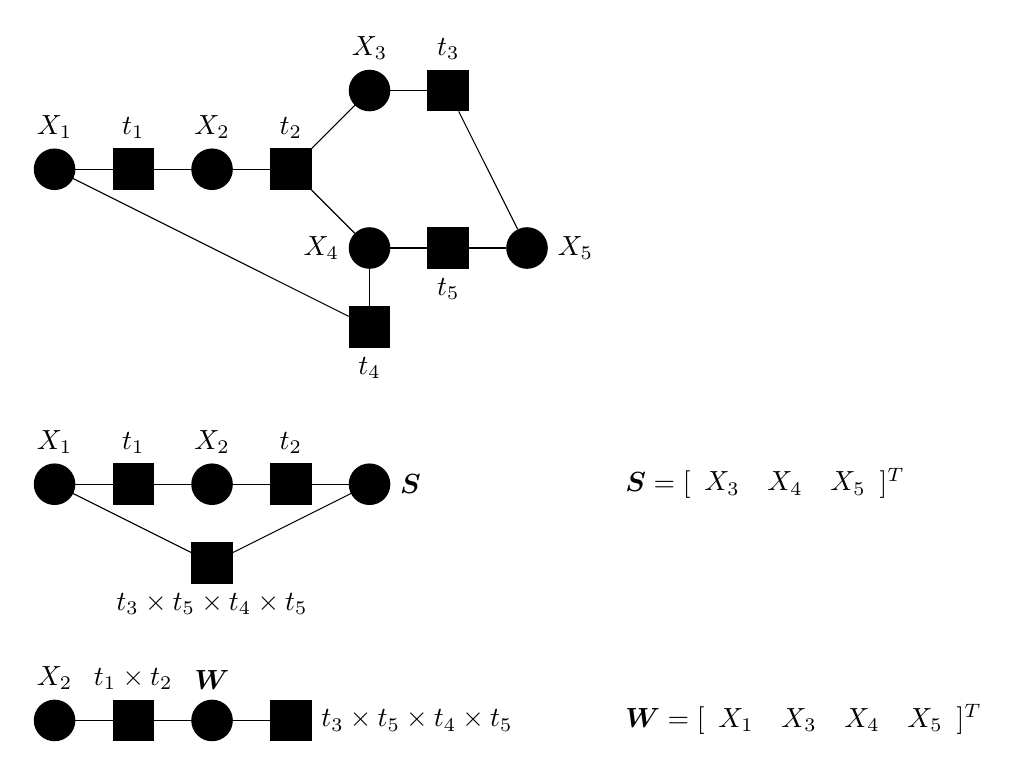
\begin{tikzpicture}[scale=1]
\tikzstyle{factor}=[rectangle,minimum size = 5mm, thick, draw =black,fill=black]
\tikzstyle{var}=[circle,minimum size = 5mm, thick, draw =black,fill=black]
\tikzstyle{second}=[circle, minimum size = 10mm, thick]
\tikzstyle{box}=[rectangle, draw=black!100]
\tikzstyle{connect}=[-latex, thick]
\draw[step=5cm];
	\node[var] (x_1) at (-1,0) [label=above:{$X_1$}]{};
	\node[factor] (t_1) at (0,0) [label=above:{$t_1$}]{};
	\node[var] (x_2) at (1,0) [label=above:{$X_2$}]{};
	\node[factor] (t_2) at (2,0) [label=above:{$t_2$}]{};
	\node[var] (x_3) at (3,1) [label=above:{$X_3$}]{};
	\node[factor] (t_3) at (4,1) [label=above:{$t_3$}]{};
	\node[var] (x_4) at (3,-1) [label=left:{$X_4$}]{};
	\node[factor] (t_4) at (3,-2) [label=below:{$t_4$}]{};
	\node[factor] (t_5) at (4,-1) [label=below:{$t_5$}]{};
	\node[var] (x_5) at (5,-1) [label=right:{$X_5$}]{};

	\node[] () at (6,-4) [label=right:{$\S=[\begin{array}{ccc} X_3 & X_4 & X_5 \end{array}]^T$}]{};
	
	\node[var] (x_12) at (-1,-4) [label=above:{$X_1$}]{};
	\node[factor] (t_12) at (0,-4) [label=above:{$t_1$}]{};
	\node[var] (x_22) at (1,-4) [label=above:{$X_2$}]{};
	\node[factor] (t_22) at (2,-4) [label=above:{$t_2$}]{};
	\node[var] (s2) at (3,-4) [label=right:{$\S$}]{};
	\node[factor] (t_s2) at (1,-5) [label=below:{$t_3\times t_5 \times t_4 \times t_5$}]{};

	\node[var] (x_23) at (-1,-7) [label=above:{$X_2$}]{};
	\node[factor] (t_w) at (0,-7) [label=above:{$t_1\times t_2$}]{};
	\node[var] (w) at (1,-7) [label=above:{$\ve{W}$}]{};
	\node[factor] (w) at (2,-7) [label=right:{$t_3\times t_5 \times t_4 \times t_5$}]{};

	\node[] () at (6,-7) [label=right:{$\ve{W}=[\begin{array}{cccc} X_1 & X_3 & X_4 & X_5 \end{array}]^T$}]{};

	\path
		(x_1) edge []  (t_2) 
		(t_2) edge [] (x_3) 
		(x_3) edge [] (t_3)
		(t_2) edge [] (x_4)
		(t_4) edge [] (x_4)
		(x_4) edge [] (x_5)
		(t_3) edge [] (x_5)
		(x_1) edge [] (t_4)
		(x_12) edge[] (s2)
		(x_12) edge [] (t_s2)
		(t_s2) edge[] (s2)
		(x_23) edge[] (w);
		
\end{tikzpicture}
\end{center}


}

\frame{

\begin{center}
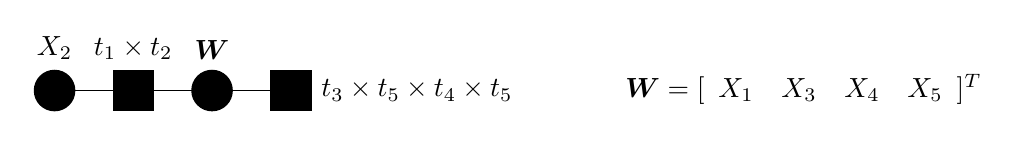
\begin{tikzpicture}[scale=1]
\tikzstyle{factor}=[rectangle,minimum size = 5mm, thick, draw =black,fill=black]
\tikzstyle{var}=[circle,minimum size = 5mm, thick, draw =black,fill=black]
\tikzstyle{second}=[circle, minimum size = 10mm, thick]
\tikzstyle{box}=[rectangle, draw=black!100]
\tikzstyle{connect}=[-latex, thick]
\draw[step=5cm];
		\node[var] (x_23) at (-1,-7) [label=above:{$X_2$}]{};
	\node[factor] (t_w) at (0,-7) [label=above:{$t_1\times t_2$}]{};
	\node[var] (w) at (1,-7) [label=above:{$\ve{W}$}]{};
	\node[factor] (w) at (2,-7) [label=right:{$t_3\times t_5 \times t_4 \times t_5$}]{};

	\node[] () at (6,-7) [label=right:{$\ve{W}=[\begin{array}{cccc} X_1 & X_3 & X_4 & X_5 \end{array}]^T$}]{};
	
	
	\path
		(x_23) edge[] (w);
		
\end{tikzpicture}
\end{center}

\begin{exampleblock}{}
BP is exact!
\end{exampleblock}

\begin{alertblock}{Increased complexity}
Computing the message
\begin{align*}
\displaystyle\mes{t_1\times t_2}{x_2}(x_2)=\sum_{\ve{w}}~ t_1(\ve{w},x_2)  t_2(\ve{w},x_2) 
\end{align*}
requires $\mathcal{O}(|\set{X}|^4)$ operations.
\end{alertblock}

\begin{block}{}
For high-dimensional, high-density graphs  $\rightarrow \mathcal{O}(|\set{X}|^{\alpha n} )$ complexity.
\end{block}


}

\subsection{Cutset conditioning}

\frame{
\frametitle{Cutset conditioning}

\begin{itemize}
\item An alternative to clustering that seeks to solve inference over a graph with cycles by working with cycle-free graphs.
\item It can be used in conjuntion to clustering.
\item For high-dimensional, high-density graphs  $\rightarrow \mathcal{O}(|\set{X}|^{\alpha n} )$ complexity.
\end{itemize}


}

\frame{



\begin{align*}
\p{\X}(\x)=\frac{1}{Z} t_1(x_1,x_2) t_2(x_2,x_3,x_4) t_3(x_3,x_5)t_4(x_4)t_5(x_4,x_5), \qquad \x\in\set{X}^5
\end{align*}

\begin{center}
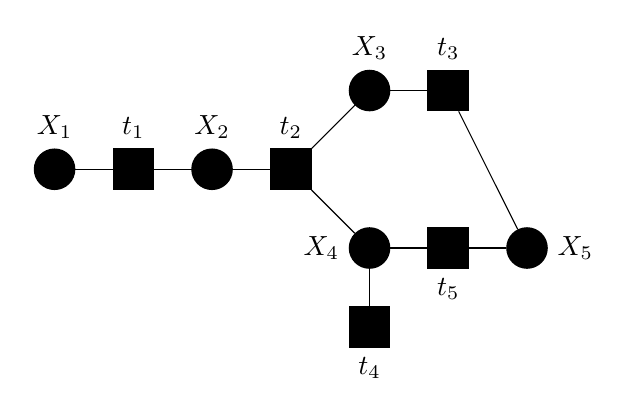
\begin{tikzpicture}[scale=1]
\tikzstyle{factor}=[rectangle,minimum size = 5mm, thick, draw =black,fill=black]
\tikzstyle{var}=[circle,minimum size = 5mm, thick, draw =black,fill=black]
\tikzstyle{second}=[circle, minimum size = 10mm, thick]
\tikzstyle{box}=[rectangle, draw=black!100]
\tikzstyle{connect}=[-latex, thick]
\draw[step=5cm];
	\node[var] (x_1) at (-1,0) [label=above:{$X_1$}]{};
	\node[factor] (t_1) at (0,0) [label=above:{$t_1$}]{};
	\node[var] (x_2) at (1,0) [label=above:{$X_2$}]{};
	\node[factor] (t_2) at (2,0) [label=above:{$t_2$}]{};
	\node[var] (x_3) at (3,1) [label=above:{$X_3$}]{};
	\node[factor] (t_3) at (4,1) [label=above:{$t_3$}]{};
	\node[var] (x_4) at (3,-1) [label=left:{$X_4$}]{};
	\node[factor] (t_4) at (3,-2) [label=below:{$t_4$}]{};
	\node[factor] (t_5) at (4,-1) [label=below:{$t_5$}]{};
	\node[var] (x_5) at (5,-1) [label=right:{$X_5$}]{};
	
	
	\path
		(x_1) edge []  (t_2) 
		(t_2) edge [] (x_3) 
		(x_3) edge [] (t_3)
		(t_2) edge [] (x_4)
		(t_4) edge [] (x_4)
		(x_4) edge [] (x_5)
		(t_3) edge [] (x_5);
		
\end{tikzpicture}
\end{center}

\begin{align*}
\set{X}=\{\mathtt{a}_1,\mathtt{a}_2,\ldots,\mathtt{a}_{|\set{X}|}\}
\end{align*}


}

\frame{




\begin{align*}
&\p{\X}(x_1,x_2,x_3=\a_1,x_4,x_5)\\
&=\frac{1}{Z} t_1(x_1,x_2) t_2(x_2,x_3=\a_1,x_4) t_3(x_3=\a_1,x_5)t_4(x_4)t_5(x_4,x_5), \qquad \x\in\set{X}^5
\end{align*}

\begin{center}
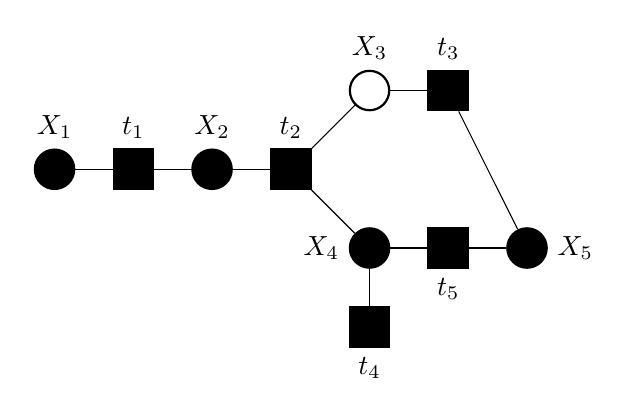
\begin{tikzpicture}[scale=1]
\tikzstyle{factor}=[rectangle,minimum size = 5mm, thick, draw =black,fill=black]
\tikzstyle{var}=[circle,minimum size = 5mm, thick, draw =black,fill=black]
\tikzstyle{varobv}=[circle,minimum size = 5mm, thick, draw =black,fill=white]
\tikzstyle{second}=[circle, minimum size = 10mm, thick]
\tikzstyle{box}=[rectangle, draw=black!100]
\tikzstyle{connect}=[-latex, thick]
\draw[step=5cm];
	\node[var] (x_1) at (-1,0) [label=above:{$X_1$}]{};
	\node[factor] (t_1) at (0,0) [label=above:{$t_1$}]{};
	\node[var] (x_2) at (1,0) [label=above:{$X_2$}]{};
	\node[factor] (t_2) at (2,0) [label=above:{$t_2$}]{};
	\node[varobv] (x_3) at (3,1) [label=above:{$X_3$}]{};
	\node[factor] (t_3) at (4,1) [label=above:{$t_3$}]{};
	\node[var] (x_4) at (3,-1) [label=left:{$X_4$}]{};
	\node[factor] (t_4) at (3,-2) [label=below:{$t_4$}]{};
	\node[factor] (t_5) at (4,-1) [label=below:{$t_5$}]{};
	\node[var] (x_5) at (5,-1) [label=right:{$X_5$}]{};
	
	
	\path
		(x_1) edge []  (t_2) 
		(t_2) edge [] (x_3) 
		(x_3) edge [] (t_3)
		(t_2) edge [] (x_4)
		(t_4) edge [] (x_4)
		(x_4) edge [] (x_5)
		(t_3) edge [] (x_5);
		
\end{tikzpicture}
\end{center}

\begin{exampleblock}{}
$\p{\X}(x_1,x_2,x_3=\a_1,x_4,x_5)$ maps over a cycle-free FG!
\end{exampleblock}

}

\frame{


\begin{center}
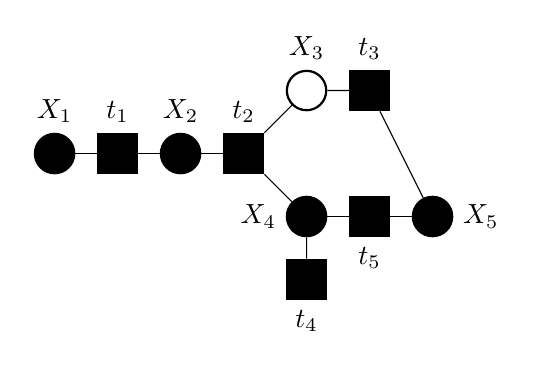
\begin{tikzpicture}[scale=0.8]
\tikzstyle{factor}=[rectangle,minimum size = 5mm, thick, draw =black,fill=black]
\tikzstyle{var}=[circle,minimum size = 5mm, thick, draw =black,fill=black]
\tikzstyle{varobv}=[circle,minimum size = 5mm, thick, draw =black,fill=white]
\tikzstyle{second}=[circle, minimum size = 10mm, thick]
\tikzstyle{box}=[rectangle, draw=black!100]
\tikzstyle{connect}=[-latex, thick]
\draw[step=5cm];
	\node[var] (x_1) at (-1,0) [label=above:{$X_1$}]{};
	\node[factor] (t_1) at (0,0) [label=above:{$t_1$}]{};
	\node[var] (x_2) at (1,0) [label=above:{$X_2$}]{};
	\node[factor] (t_2) at (2,0) [label=above:{$t_2$}]{};
	\node[varobv] (x_3) at (3,1) [label=above:{$X_3$}]{};
	\node[factor] (t_3) at (4,1) [label=above:{$t_3$}]{};
	\node[var] (x_4) at (3,-1) [label=left:{$X_4$}]{};
	\node[factor] (t_4) at (3,-2) [label=below:{$t_4$}]{};
	\node[factor] (t_5) at (4,-1) [label=below:{$t_5$}]{};
	\node[var] (x_5) at (5,-1) [label=right:{$X_5$}]{};
	
	
	\path
		(x_1) edge []  (t_2) 
		(t_2) edge [] (x_3) 
		(x_3) edge [] (t_3)
		(t_2) edge [] (x_4)
		(t_4) edge [] (x_4)
		(x_4) edge [] (x_5)
		(t_3) edge [] (x_5);
		
\end{tikzpicture}
\end{center}


\begin{block}{}
Using BP, we can compute
\begin{align*}
&\p{X_3}(x_3=\a_1)\\
&\p{X_1,X_3}(x_1,x_3=\a_1)\\
&\p{X_2,X_3}(x_2,x_3=\a_1)\\
&\p{X_4,X_3}(x_4,x_3=\a_1)\\
&\p{X_5,X_3}(x_5,x_3=\a_1)\\
\end{align*}
at cost \noteB{$\mathcal{O}(n|\set{X}|^3)$}.
\end{block}


}

\frame{
We can proceed similarly to compute 
\begin{align*}
&\p{X_3}(x_3=\a_j)\\
&\p{X_i,X_3}(x_i,x_3=\a_j)
\end{align*}
for all $a_j\in\set{X}$ and $i=1,2,4,5$.  The marginal for $X_3$ is already computed, and the rest of marginals...
\begin{align*}
\p{X_i}(x_i)=\sum_{x_3\in\set{X}} \p{X_i,X_3}(x_i,x_3)
\end{align*}

\begin{block}{For a single cycle, the overall complexity is ...}
\centering\noteB{$\mathcal{O}(n |\set{X}|^3 \times \color{red}{|\set{X}|}\color{black}{})$}
\end{block}

\begin{alertblock}{For a high-dimensional, high-density graph the \# of cycles is proportional to n}
\centering\noteB{$\mathcal{O}(n|\set{X}|^d\times \color{red}{|\set{X}|^{\alpha n}}\color{black}{})$}
\end{alertblock}

}

\section{The Junction Tree Algorithm}

\frame{
\frametitle{Just some words about the Junction Tree Algorithm (JTA)}

\begin{itemize}
\item Systematic procedure to perform \noteG{exact inference} over arbitrary graphs.
\item Construct tree-graph representations of our graph via clustering.
\item Given the FG of our problem, we construct a \noteB{cluster graph} with the properties of a \noteR{junction tree.}
\item Run a generalization of BP over cluster graphs. Exact for a junction tree!
\end{itemize}

\begin{alertblock}{}
In a great deal of interesting applications the use of the JTA algorithm would result in clusters  that are prohibitively large. \noteB{$\mathcal{O}(|\set{X}|^{\alpha n})$} complexity.
\end{alertblock}

\begin{exampleblock}{JTA complexity is typically affordable for highly regular graphs!}
\begin{itemize}
\item Hidden Markov model, state-space models.
\item Lattice-models (widely used in image statistical modelling ...)
\end{itemize}
\end{exampleblock}

\noteB{Take a look of Chapter 6, David Barber's book!}.

}

\section{Loopy BP}

\frame{
\frametitle{The need for approximations}

\begin{itemize}
\item For many problems of practical interest, it will not be feasible to use exact inference (JTA).
\item We need to exploit effective approximation methods.
\begin{itemize}
\item \noteB{Deterministic approaches.} Variational methods.
\item \noteG{Monte Carlo methods}. Based on stochastic numerical sampling.
\end{itemize}
\item Simplest approximate inference method: \noteB{loopy-BP}.
\end{itemize}


}

\frame{
\frametitle{Loopy Belief Propagation}
\begin{itemize}
\item Apply the exact same BP rules, ignoring the fact that the FG may contain cycles.
\end{itemize}
\begin{itemize}
\item Not a problem   because the BP message passing rules are purely local.
\end{itemize}
\begin{itemize}
\item An  ``iterative" algorithm with no natural termination will result. Messages passed multiple times on a given edge.
\end{itemize}
\begin{itemize}
\item \noteR{Convergence is not guaranteed}. For some models, BP converges for some others not. 
\end{itemize}

\begin{exampleblock}{\noteB{Global initialization}}
  We set  all the initial messages from variables to 1.
\begin{align*}
\text{For all variable nodes: }~~ &\mes{x_i}{t_j}(x_i)=1~~ x_i\in\set{X}
\end{align*}
\end{exampleblock}


}

\frame{


\begin{center}
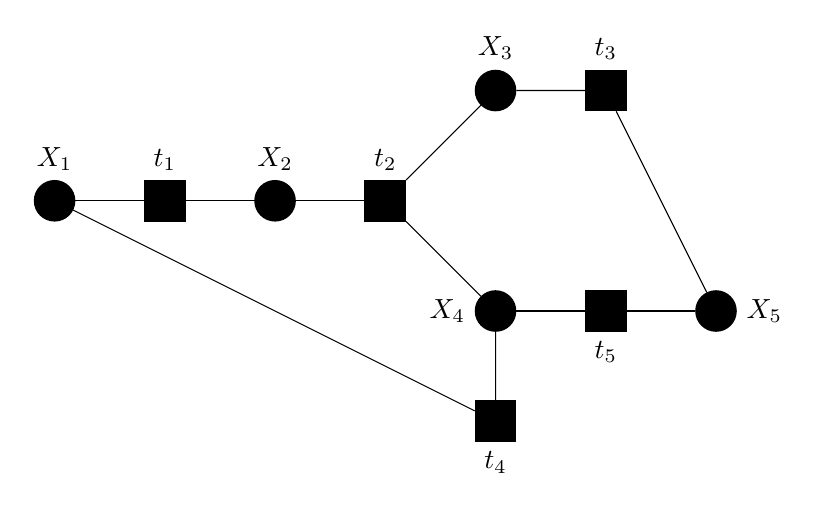
\begin{tikzpicture}[scale=1.4]
\tikzstyle{factor}=[rectangle,minimum size = 5mm, thick, draw =black,fill=black]
\tikzstyle{var}=[circle,minimum size = 5mm, thick, draw =black,fill=black]
\tikzstyle{second}=[circle, minimum size = 10mm, thick]
\tikzstyle{box}=[rectangle, draw=black!100]
\tikzstyle{connect}=[-latex, thick]
\draw[step=5cm];
	\node[var] (x_1) at (-1,0) [label=above:{$X_1$}]{};
	\node[factor] (t_1) at (0,0) [label=above:{$t_1$}]{};
	\node[var] (x_2) at (1,0) [label=above:{$X_2$}]{};
	\node[factor] (t_2) at (2,0) [label=above:{$t_2$}]{};
	\node[var] (x_3) at (3,1) [label=above:{$X_3$}]{};
	\node[factor] (t_3) at (4,1) [label=above:{$t_3$}]{};
	\node[var] (x_4) at (3,-1) [label=left:{$X_4$}]{};
	\node[factor] (t_4) at (3,-2) [label=below:{$t_4$}]{};
	\node[factor] (t_5) at (4,-1) [label=below:{$t_5$}]{};
	\node[var] (x_5) at (5,-1) [label=right:{$X_5$}]{};

	%\node[] () at (-0.9,0.2) [label=right:{$\color{darkred}\mathbf{\ve{1}\rightarrow}$}]{};
	%\node[] () at (0.2,0.2) [label=right:{$\color{darkred}\mathbf{\leftarrow \ve{1}}$}]{};

	\path
		(x_1) edge []  (t_2) 
		(t_2) edge [] (x_3) 
		(x_3) edge [] (t_3)
		(t_2) edge [] (x_4)
		(t_4) edge [] (x_4)
		(x_4) edge [] (x_5)
		(t_3) edge [] (x_5)
		(x_1) edge [] (t_4);
		
\end{tikzpicture}
\end{center}


}


\frame{
\frametitle{Global Initialization}

\begin{itemize}
\item $\color{darkred}\ve{1}\rightarrow$: all-1s message.
\end{itemize}

\begin{center}
\begin{tikzpicture}[scale=1.4]
\tikzstyle{factor}=[rectangle,minimum size = 5mm, thick, draw =black,fill=black]
\tikzstyle{var}=[circle,minimum size = 5mm, thick, draw =black,fill=black]
\tikzstyle{second}=[circle, minimum size = 10mm, thick]
\tikzstyle{box}=[rectangle, draw=black!100]
\tikzstyle{connect}=[-latex, thick]
\draw[step=5cm];
	\node[var] (x_1) at (-1,0) [label=above:{$X_1$}]{};
	\node[factor] (t_1) at (0,0) [label=above:{$t_1$}]{};
	\node[var] (x_2) at (1,0) [label=above:{$X_2$}]{};
	\node[factor] (t_2) at (2,0) [label=above:{$t_2$}]{};
	\node[var] (x_3) at (3,1) [label=above:{$X_3$}]{};
	\node[factor] (t_3) at (4,1) [label=above:{$t_3$}]{};
	\node[var] (x_4) at (3,-1) [label=left:{$X_4$}]{};
	\node[factor] (t_4) at (3,-2) [label=below:{$t_4$}]{};
	\node[factor] (t_5) at (4,-1) [label=below:{$t_5$}]{};
	\node[var] (x_5) at (5,-1) [label=right:{$X_5$}]{};

	\node[] () at (-0.9,0.2) [label=right:{$\color{darkred}\mathbf{\ve{1}\rightarrow}$}]{};
	\node[] () at (0.2,0.2) [label=right:{$\color{darkred}\mathbf{\leftarrow \ve{1}}$}]{};
	\node[] () at (1.1,0.2) [label=right:{$\color{darkred}\mathbf{\ve{1}\rightarrow}$}]{};
	%\node[] () at (-0.9,-0.3) [rotate=-90,label=below:rotate,label={$\color{darkred}\mathbf{\ve{1}\rightarrow}$}]{};
	\node[rotate=-30]  at (-0.45,-0.45) {$\color{darkred}\mathbf{\ve{1}\rightarrow}$};
	\node[rotate=45]  at (2.5,0.75) {$\color{darkred}\mathbf{\leftarrow \ve{1}}$};
	\node[rotate=-45]  at (2.3,-0.5) {$\color{darkred}\mathbf{\leftarrow \ve{1}}$};
	\node[rotate=0]  at (3.5,1.2) {$\color{darkred}\mathbf{\ve{1}\rightarrow}$};
	 \node[rotate=0]  at (3.5,-0.8) {$\color{darkred}\mathbf{\ve{1}\rightarrow}$};
	 \node[rotate=270]  at (2.8,-1.5) {$\color{darkred}\mathbf{\ve{1}\rightarrow}$}; 
	 \node[rotate=0]  at (4.5,-0.8) {$\color{darkred}\mathbf{\leftarrow \ve{1}}$};
	  \node[rotate=-60]  at (5,-0.5) {$\color{darkred}\mathbf{\leftarrow \ve{1}}$};
	\path
		(x_1) edge []  (t_2) 
		(t_2) edge [] (x_3) 
		(x_3) edge [] (t_3)
		(t_2) edge [] (x_4)
		(t_4) edge [] (x_4)
		(x_4) edge [] (x_5)
		(t_3) edge [] (x_5)
		(x_1) edge [] (t_4);
		
\end{tikzpicture}
\end{center}


}

\frame{
\frametitle{Flooding scheme (I)}

\begin{itemize}
\item All factor nodes recompute a message for each neighbor. 
\end{itemize}

\begin{center}
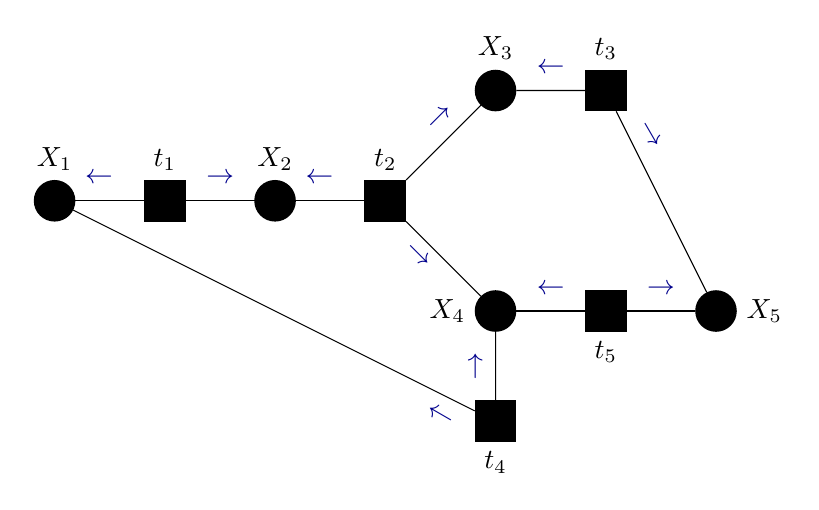
\begin{tikzpicture}[scale=1.4]
\tikzstyle{factor}=[rectangle,minimum size = 5mm, thick, draw =black,fill=black]
\tikzstyle{var}=[circle,minimum size = 5mm, thick, draw =black,fill=black]
\tikzstyle{second}=[circle, minimum size = 10mm, thick]
\tikzstyle{box}=[rectangle, draw=black!100]
\tikzstyle{connect}=[-latex, thick]
\draw[step=5cm];
	\node[var] (x_1) at (-1,0) [label=above:{$X_1$}]{};
	\node[factor] (t_1) at (0,0) [label=above:{$t_1$}]{};
	\node[var] (x_2) at (1,0) [label=above:{$X_2$}]{};
	\node[factor] (t_2) at (2,0) [label=above:{$t_2$}]{};
	\node[var] (x_3) at (3,1) [label=above:{$X_3$}]{};
	\node[factor] (t_3) at (4,1) [label=above:{$t_3$}]{};
	\node[var] (x_4) at (3,-1) [label=left:{$X_4$}]{};
	\node[factor] (t_4) at (3,-2) [label=below:{$t_4$}]{};
	\node[factor] (t_5) at (4,-1) [label=below:{$t_5$}]{};
	\node[var] (x_5) at (5,-1) [label=right:{$X_5$}]{};

	\node[] () at (-0.9,0.2) [label=right:{$\color{darkblue}\mathbf{\leftarrow}$}]{};
	\node[] () at (0.2,0.2) [label=right:{$\color{darkblue}\mathbf{\rightarrow }$}]{};
	\node[] () at (1.1,0.2) [label=right:{$\color{darkblue}\mathbf{\leftarrow}$}]{};
	%\node[] () at (-0.9,-0.3) [rotate=-90,label=below:rotate,label={$\color{darkblue}\mathbf{\ve{1}\rightarrow}$}]{};
	\node[rotate=-30]  at (2.5,-1.95) {$\color{darkblue}\mathbf{\leftarrow}$};
	\node[rotate=45]  at (2.5,0.75) {$\color{darkblue}\mathbf{\rightarrow}$};
	\node[rotate=-45]  at (2.3,-0.5) {$\color{darkblue}\mathbf{\rightarrow }$};
	\node[rotate=0]  at (3.5,1.2) {$\color{darkblue}\mathbf{\leftarrow}$};
	 \node[rotate=0]  at (3.5,-0.8) {$\color{darkblue}\mathbf{\leftarrow}$};
	 \node[rotate=270]  at (2.8,-1.5) {$\color{darkblue}\mathbf{\leftarrow}$}; 
	 \node[rotate=0]  at (4.5,-0.8) {$\color{darkblue}\mathbf{\rightarrow}$};
	  \node[rotate=-60]  at (4.4,0.6) {$\color{darkblue}\mathbf{\rightarrow}$};
	\path
		(x_1) edge []  (t_2) 
		(t_2) edge [] (x_3) 
		(x_3) edge [] (t_3)
		(t_2) edge [] (x_4)
		(t_4) edge [] (x_4)
		(x_4) edge [] (x_5)
		(t_3) edge [] (x_5)
		(x_1) edge [] (t_4);
		
\end{tikzpicture}
\end{center}



}


\frame{
\frametitle{Flooding scheme (II)}

\begin{itemize}
\item All variable nodes recompute a message for each neighbor. 
\end{itemize}

\begin{center}
\begin{tikzpicture}[scale=1.4]
\tikzstyle{factor}=[rectangle,minimum size = 5mm, thick, draw =black,fill=black]
\tikzstyle{var}=[circle,minimum size = 5mm, thick, draw =black,fill=black]
\tikzstyle{second}=[circle, minimum size = 10mm, thick]
\tikzstyle{box}=[rectangle, draw=black!100]
\tikzstyle{connect}=[-latex, thick]
\draw[step=5cm];
	\node[var] (x_1) at (-1,0) [label=above:{$X_1$}]{};
	\node[factor] (t_1) at (0,0) [label=above:{$t_1$}]{};
	\node[var] (x_2) at (1,0) [label=above:{$X_2$}]{};
	\node[factor] (t_2) at (2,0) [label=above:{$t_2$}]{};
	\node[var] (x_3) at (3,1) [label=above:{$X_3$}]{};
	\node[factor] (t_3) at (4,1) [label=above:{$t_3$}]{};
	\node[var] (x_4) at (3,-1) [label=left:{$X_4$}]{};
	\node[factor] (t_4) at (3,-2) [label=below:{$t_4$}]{};
	\node[factor] (t_5) at (4,-1) [label=below:{$t_5$}]{};
	\node[var] (x_5) at (5,-1) [label=right:{$X_5$}]{};

	\node[] () at (-0.9,0.2) [label=right:{$\color{darkred}\mathbf{\rightarrow}$}]{};
	\node[] () at (0.2,0.2) [label=right:{$\color{darkred}\mathbf{\leftarrow }$}]{};
	\node[] () at (1.1,0.2) [label=right:{$\color{darkred}\mathbf{\rightarrow}$}]{};
	%\node[] () at (-0.9,-0.3) [rotate=-90,label=below:rotate,label={$\color{darkred}\mathbf{\ve{1}\rightarrow}$}]{};
	\node[rotate=-30]  at (-0.45,-0.45) {$\color{darkred}\mathbf{\rightarrow}$};
	\node[rotate=45]  at (2.5,0.75) {$\color{darkred}\mathbf{\leftarrow }$};
	\node[rotate=-45]  at (2.3,-0.5) {$\color{darkred}\mathbf{\leftarrow}$};
	\node[rotate=0]  at (3.5,1.2) {$\color{darkred}\mathbf{\rightarrow}$};
	 \node[rotate=0]  at (3.5,-0.8) {$\color{darkred}\mathbf{\rightarrow}$};
	 \node[rotate=270]  at (2.8,-1.5) {$\color{darkred}\mathbf{\rightarrow}$}; 
	 \node[rotate=0]  at (4.5,-0.8) {$\color{darkred}\mathbf{\leftarrow}$};
	  \node[rotate=-60]  at (5,-0.5) {$\color{darkred}\mathbf{\leftarrow}$};
	\path
		(x_1) edge []  (t_2) 
		(t_2) edge [] (x_3) 
		(x_3) edge [] (t_3)
		(t_2) edge [] (x_4)
		(t_4) edge [] (x_4)
		(x_4) edge [] (x_5)
		(t_3) edge [] (x_5)
		(x_1) edge [] (t_4);
		
\end{tikzpicture}
\end{center}

\begin{alertblock}{}
There is no guarantee that this update rules converge to a fixed point.  In practice, all schedules are finite, either by running the algorithm for a finite-number of iterations or by another termination condition.
\end{alertblock}

}

\frame{
\frametitle{Approximated marginals}

\begin{itemize}
\item Upon finalization,  marginals are estimated using the product of the most recently received incoming messages to each variable node. 
\end{itemize}

\begin{align*}
\p{X_i}(x_i)\approx \frac{1}{Z_i}\prod_{k\in\Iset{Ne}(X_i)}\mes{t_k}{x_i}(x_i),
\end{align*}

\begin{itemize}
\item In some applications,  loopy BP can give poor results, where in other applications it has proven to be very effective.
\end{itemize}

\begin{itemize}
\item \noteG{LDPC decoding}.
\item \noteG{Signal reconstruction in compressed sensing applications}.
\item \noteG{Symbol detection in massive MIMO scenarios}.
\item ...
\end{itemize}


}

\frame{
\frametitle{Analysis of Loopy-BP}

Several works have yielded insight into the dynamics and convergence properties of loopy BP:

\begin{exampleblock}{}
\noteB{Weiss, Y. (1997). Belief propagation and revision in networks with loops.
Technical report, Cambridge, MA, USA.}
\begin{itemize}
\item For graphs with a \noteR{single-cycle}, it has
been proven that the loopy BP always converges to a fixed point that can be analytically characterized.
\end{itemize}
\begin{itemize}
\item Further, if the hidden variables in the cycle are binary-valued, then a decisor based on the approximate
marginals computed by loopy BP is equivalent to the MAP solution.
\end{itemize}
\end{exampleblock}

}

\frame{
\frametitle{Analysis of Loopy-BP}

Several works have yielded insight into the dynamics and convergence properties of loopy BP:

\begin{exampleblock}{}
\noteB{Weiss, Y. and Freeman, W. T. Correctness of belief
propagation in gaussian graphical models of arbitrary topology. NIPS 1999.}
\begin{itemize}
\item BP algorithm applied to a \noteG{Gaussian} pdf  that maps over a cycle-free
FG provides the exact marginals with a \noteR{complexity cubic in the cluster size}. 
\end{itemize}
\begin{itemize}
\item Sufficient conditions for convergence of  BP when the algorithm converges it gives the \noteG{exact posterior means} for all graph topologies, not just cycle-free FGs.
\end{itemize}
\end{exampleblock}

}

\frame{
\frametitle{Analysis of Loopy-BP}

Several works have yielded insight into the dynamics and convergence properties of loopy BP:

\begin{exampleblock}{}
\noteB{Yedidia, J. S., Freeman, W. T., and Weiss, Y. Generalized
belief propagation. NIPS 2001.}
\begin{itemize}
\item Fixed
points of the loopy belief propagation are actually \noteB{stationary points of the Bethe free
energy} from statistical physics.
\end{itemize}
\begin{itemize}
\item The Bethe free energy provides a firm \noteR{theoretical basis
of loopy belief propagation} and it served as a basis for more advanced methods, such as
generalized belief propagation.
\end{itemize}
\end{exampleblock}

}


%
%\frame{
%\frametitle{Sparse FGs: an example}
%
%Consider a distribution of the form
%\begin{align*}
%\p{\X}(\x)\propto \prod_{j\in\Iset{J}}t_j(\x_{j}) \qquad x_i\in\set{X},~~ i=1,\ldots,n
%\end{align*}
%where each $t_j$ factor is only connected to 3 variable nodes chosen at random from $\{X_1,X_2,\ldots,X_n\}$ and each variable node $X_i$ is only connected to 2 factor nodes.
%
%\begin{itemize}
%\item The graph has $2n$ edges.
%\item $\frac{2}{3}n$ factor nodes.
%\item Connections are perform at random according to these constraints.
%\item Note that we are not defining a specific graph but an \emph{ensemble} of graphs.
%\end{itemize}
%
%
%}
%
%\frame{
%Example for $n=6$ ...
%
%
%\begin{center}
%\begin{tikzpicture}[scale=1.4]
%\tikzstyle{factor}=[rectangle,minimum size = 5mm, thick, draw =black,fill=black]
%\tikzstyle{var}=[circle,minimum size = 5mm, thick, draw =black,fill=black]
%\tikzstyle{second}=[circle, minimum size = 10mm, thick]
%\tikzstyle{box}=[rectangle, draw=black!100]
%\tikzstyle{connect}=[-latex, thick]
%\draw[step=5cm];
%
%	\draw[double](0,0)--(1,-2);
%	\node[var] (x_1) at (0,0) []{};
%	\node[var] (x_2) at (1,0) []{};
%	\node[var] (x_3) at (2,0) []{};
%	\node[var] (x_4) at (3,0) []{};
%	\node[var] (x_5) at (4,0) []{};
%	\node[var] (x_6) at (5,0) []{};
%	
%	\node[factor] (t_1) at (1,-2) []{};
%	\node[factor] (t_2) at (2,-2) []{};
%	\node[factor] (t_3) at (3,-2) []{};
%	\node[factor] (t_4) at (4,-2) []{};
%	
%	
%\path
%		(t_1) edge []  (x_3) 
%		(t_2) edge []  (x_2)
%		(t_2) edge []  (x_5)
%		(t_2) edge []  (x_6)
%		(t_3) edge []  (x_2)
%		(t_3) edge []  (x_3)	
%		(t_3) edge []  (x_4)
%		(t_4) edge []  (x_4)
%		(t_4) edge []  (x_5)	
%		(t_4) edge []  (x_6);
%		
%\end{tikzpicture}
%\end{center}
%
%\begin{block}{}
%This graph obviously has cycles.
%\end{block}
%
%\begin{exampleblock}{The ``tree''-local graph}
%Select one variable node and compute the probability in the ensemble of all possible local graphs up to a depth of $L$ jumps, $L=1, 2, 3\ldots$. 
%\end{exampleblock}
%
%
%}
%
%\frame{
%\frametitle{$L=1$ or how many factor nodes I'm connected to}
%
%
%\begin{center}
%\begin{tikzpicture}[scale=1.4]
%\tikzstyle{factor}=[rectangle,minimum size = 5mm, thick, draw =black,fill=black]
%\tikzstyle{var}=[circle,minimum size = 5mm, thick, draw =black,fill=black]
%\tikzstyle{second}=[circle, minimum size = 10mm, thick]
%\tikzstyle{box}=[rectangle, draw=black!100]
%\tikzstyle{connect}=[-latex, thick]
%\draw[step=5cm];
%
%	
%	\draw[double](0,0)--(0,-1);
%	\draw (0,-1) -- (0,-1.5);
%	
%	\node[var] (x_1) at (0,0) []{};
%	\node[factor] (t_1) at (0,-1) []{};
%	
%	\draw (-0.5,-3)--(-0.8,-3.5);
%	\draw (-0.5,-3)--(-0.2,-3.5);
%	
%	\draw (0.5,-3)--(0.8,-3.5);
%	\draw (0.5,-3)--(0.2,-3.5);
%	\node[var] (x_2) at (0,-2) []{};
%	\node[factor] (t_2) at (-0.5,-3)[] {};
%	\node[factor] (t_3) at (0.5,-3)[] {};
%	
%	\path
%		(x_2) edge [] (t_2)
%		(x_2) edge [] (t_3);
%		
%	\node[] () at (1, 1) [label=right:{Probability in a randomly generated graph}]{};		
%	\node[] () at (3,-0.5) [label=right:{$\frac{2}{2n-1}$}]{};
%	\node[] () at (3,-2.5) [label=right:{$\frac{2n-3}{2n-1}$}]{};
%		
%\end{tikzpicture}
%\end{center}
%
%
%}
%
%\frame{
%\frametitle{$L=2$ or how many variable nodes I can reach in 2 jumps}
%
%\begin{center}
%\begin{tikzpicture}[scale=0.8]
%\tikzstyle{factor}=[rectangle,minimum size = 3mm, thick, draw =black,fill=black]
%\tikzstyle{var}=[circle,minimum size = 3mm, thick, draw =black,fill=black]
%\tikzstyle{second}=[circle, minimum size = 10mm, thick]
%\tikzstyle{box}=[rectangle, draw=black!100]
%\tikzstyle{connect}=[-latex, thick]
%\draw[step=5cm];
%
%	
%	\draw(-0.02,1)--(-0.02,0) {};
%	\draw(0.02,1)--(0.02,0) {}; 
%	\draw (0,0) -- (0,-1);
%	
%	\node[var] (x_1) at (0,1) []{};
%	\node[factor] (t_1) at (0,0) []{};
%	\node[var] (x_12) at (0,-1) []{};
%	
%	\draw(3.52,0)--(3.52,-1) {};
%	\draw(3.48,0)--(3.48,-1) {};
%	\draw(4.52,0)--(4.52,-1) {};
%	\draw(4.48,0)--(4.48,-1) {};
%	
%	
%	\node[var] (x_7) at (4,1) []{};
%	\node[factor] (t_7) at (3.5,0) []{};
%	\node[factor] (t_8) at (4.5,0) []{};
%	\node[var] (x_8) at (3.5,-1) []{};
%	\node[var] (x_9) at (4.5,-1) []{}; 
%	
%	\path 
%		(x_7) edge [] (t_7)
%		(x_7) edge [] (t_8);
%	
%	
%		\draw(3.52,-3)--(3.52,-4) {};
%	\draw(3.48,-3)--(3.48,-4) {};
%	\draw(4.5,-3)--(4.2,-4) {};
%	\draw(4.5,-3)--(4.8,-4) {};
%	
%	
%	\node[var] (x_10) at (4,-2) []{};
%	\node[factor] (t_10) at (3.5,-3) []{};
%	\node[factor] (t_11) at (4.5,-3) []{};
%	\node[var] (x_11) at (3.5,-4) []{};
%	\node[var] (x_12a) at (4.2,-4) []{};
%	\node[var] (x_12b) at (4.8,-4) []{};
%	
%	\path 
%		(x_10) edge [] (t_10)
%		(x_10) edge [] (t_11);
%	
%	\node[var] (x_2) at (0,-2) []{};
%	\node[factor] (t_2) at (-0.5,-3)[] {};
%	\node[factor] (t_3) at (0.5,-3)[] {};
%	\node[var] (x_3) at (0.8,-4) []{};
%	\node[var] (x_4) at (0.2,-4) []{};
%	\node[var] (x_5) at (-0.8,-4) []{};
%	\node[var] (x_6) at (-0.2,-4) []{};
%	
%	\path
%		(x_2) edge [] (t_2)
%		(x_2) edge [] (t_3)
%		(t_3) edge [] (x_3)
%		(t_3) edge [] (x_4)
%		(t_2) edge [] (x_5)
%		(t_2) edge [] (x_6);		
%		
%	\node[var] (x_a) at (0,-5) []{};
%	\node[factor] (t_a) at (-0.5,-6)[] {};
%	\node[factor] (t_b) at (0.5,-6)[] {};
%	\node[var] (x_b) at (1,-7) []{};
%	\node[var] (x_c) at (0,-7) []{};
%	\node[var] (x_d) at (-1,-7) []{};
%
%	
%	\path
%		(x_a) edge [] (t_a)
%		(x_a) edge [] (t_b)
%		(t_b) edge [] (x_b)
%		(t_b) edge [] (x_c)
%		(t_a) edge [] (x_c)
%		(t_a) edge [] (x_d);			
%		
%		
%	\node[var] (x_aa) at (4,-5) []{};
%	\node[factor] (t_aa) at (3.5,-6)[] {};
%	\node[factor] (t_bb) at (4.5,-6)[] {};
%	\node[var] (x_bb) at (3.5,-7) []{};
%	\node[var] (x_cc) at (4.5,-7) []{};
%	
%
%	
%	\path
%		(x_aa) edge [] (t_aa)
%		(x_aa) edge [] (t_bb)
%		(t_bb) edge [] (x_bb)
%		(t_bb) edge [] (x_cc)
%		(t_aa) edge [] (x_cc)
%		(t_aa) edge [] (x_bb);			
%			
%	\node[] () at (-4,0) [label=right:{$\frac{2}{2n-1}$}]{};
%	\node[] () at (-4,-3) [label=right:{$\frac{(2n-6)(2n-8)}{(2n-1)(2n-5)}$}]{};
%	\node[] () at (-4,-6) [label=right:{$\frac{4(2n-6)}{(2n-1)(2n-5)}$}]{};
%	
%	\node[] () at (6,0) [label=right:{$\frac{1}{(2n-1)(2n-5)}$}]{};
%	\node[] () at (6,-3) [label=right:{$\frac{2(2n-6)}{(2n-1)(2n-5)}$}]{};
%	\node[] () at (6,-6) [label=right:{$\frac{2}{(2n-1)(2n-5)}$}]{};
%%		
%\end{tikzpicture}
%\end{center}
%
%}
%
%
%\frame{
%
%\begin{itemize}
%\item For sufficiently large $n$, the most likely scenario is a ``local''-tree graph! 
%\item Suitable for BP approximate inference!
%\end{itemize}
%
%\begin{alertblock}{BP for dense graphs}
%While in the discrete case BP is essentially restricted to sparse graphical models (that locally look like a tree), for continuous distributions BP can provide a sensible approximation even for very dense graphs. 
%
%\vspace{0.5cm}
%For instance, we will see that BP over Gaussian factor graphs provides the \noteB{exact mean} for each variable in the graph regardeless the graph topology!
%\end{alertblock}
%
%}

\end{document}

